\begin{abstract}
	Questo articolo riassume con delle carte mnemoniche gli argomenti di farmacologia spiegati nel IV anno del corso di laurea in medicina e chirurgia a Chieti.
	L'uso di questo articolo non sostituisce la lettura e lo studio di un libro e degli appunti di farmacologia.
	Per errori, omissioni o altre note, non esitate a contattarmi via e-mail.
\end{abstract}

\newpage\newpage

\section{Farmaci del SNC e del SNP}

\begin{tikzpicture}
	\itm{snc}{Sistema nervoso};
	\itmsplit{snc}{orto}{Simpatico\\ (toraco--addominale)}{para}{Parasimpatico \\(nervi crani e sacrale)}
	\itmr{}{nell'intima degli organi}
	\itmrights{orto}{}{gangli pre e para--vertebrali}
\end{tikzpicture}

\begin{tikzpicture}
	\itm{main}{Neurotrasmettitori};
	\itmsplitfour{main}{a}{acetilcolina}{b}{noradrenalina}{c}{serotonina}{d}{monossido d'azoto (NO)}
	\itmrights{a}{}{recettori colinergici};
	\itmrights{b}{}{recettori adrenergici};
	\itmrights{c}{}{recettori serotoninergici};
	\node[itm, below=4.5em of c] (purine) {purine};
	\draw[thick,shorten <=2pt] (main.east) -- ++(.3,0) [shorten >=2pt,shorten <=0pt,->] to[out=-45,in=125] (purine.north west);
\end{tikzpicture}

\subsection{Acetilcolina}

\begin{tikzpicture}
	\itm{mainh}{acetilcolina};
	\itmsplitfour{mainh}{a}{tutte le fibre pregangliali sia pra che orto}{b}{parasimpatiche post gangliali (quasi tutte). Tipo muscarinico}{c}{qualche simpatico postgangliare soprattutto ghiandole sudoripare}{d}{giunzione neuromuscolare}
\end{tikzpicture}

\begin{tikzpicture}
	\itm{main}{Sintesi};
	\itmr{a}{acetilCOA + colina}
	\dummyzar{a}
	\itmr{b}{acetilcolina}
	
	\node[above right=-.5em and 1em of a] {colina};
	\node[below right=-.5em and 0em of a] {acetiltrasferasi};
\end{tikzpicture}

\begin{tikzpicture}
	\itm{main}{Degradazione};
	\itmr{a}{acetilcolina}
	\dummyzar{a}
	\itmr{b}{acetato + colina}
	\node[below right=-.5em and -.3em of a] {acetilcolinesterasi};
\end{tikzpicture}

\begin{tikzpicture}
	\itm{main}{Recettore colinergico\\ (ionotropo)};
	\dummy{main};
	\itmabove{main_dummy}{muscarinico}{muscarinico\\ (proteine G)}{main};
	\node[itm, below=10em of main_dummy] (nicotinico) {nicotinico\\ (canale)};
	\draw[thick,shorten >=2pt,->] ($(main.east) + (.3,0)$)  to[out=-45,in=155] (nicotinico.north west);
	\itmsplitfour{muscarinico}{a}{M${}_1\, \uparrow\text{IP}_3, \text{Ca}^{2+}$ eccitatorio (SNC, simpatico post--gangliare)}{b}{M${}_2\, \downarrow$cAMP inibitorio (cuore)}{c}{M${}_3\, \uparrow\text{IP}_3$ eccitatorio (ghiandole esocrine)}{d}{M${}_4$ eccitatorio (SNC)}
	\node[itm, below=4.5em of c] (e) {M${}_5$ eccitatorio (endotelio vasale)};
	\draw[thick,shorten <=2pt] (muscarinico.east) -- ++(.3,0) [shorten >=2pt,shorten <=0pt,->] to[out=-45,in=155] (e.north west);
	
	\itmsplit{nicotinico}{f}{N${}_\text{N}$ para e\\ ortosimpatico gangliare}{g}{N${}_\text{M}$ giunzione\\ neuromuscolare};
\end{tikzpicture}

\subsection{Noradrenalina}

\begin{tikzpicture}
	\itm{main}{noradrenalina};
	\itmr{}{simpatiche postgangliari}
\end{tikzpicture}

\begin{tikzpicture}
	\itm{main}{Sintesi};
	\itmr{a}{Tirosina}
	\dummyzar{a}
	\itmr{b}{DOPA}
	\itmr{c}{dopamina}
	\itmr{d}{noradrenalina}
	\dummyend{d}
	
	\dummystart{e}{main}
	\itmr{f}{adrenalina}
	
	\node[above right=-.5em and -.2em of a] {tirosin--idrossilasi};
	\node[below right=-.5em and 0em of a] {tappa limitante};
\end{tikzpicture}

\begin{tikzpicture}
	\itm{maina}{Degradazione};
	\itmsplit{maina}{x}{MAO in fegato e cellule ?????}{y}{COMT nei neuroni}
\end{tikzpicture}

\begin{tikzpicture}
	\itm{main}{Recettore adrenergico\\ (metabotropo \\ a proteine G)};
	\itmsplit{main}{a}{$\alpha$}{b}{$\beta$};
	\itmsplit{a}{c}{$\alpha_1\,\text{G}_{\text{q}} \uparrow\text{IP}_3, \uparrow\text{Ca}^{2+}$ (postsinaptiche muscolo liscio) }{d}{$\alpha_2\,\text{G}_{\text{i}} \downarrow\text{cAMP}$ (presinaptiche muscolo liscio) };
	\itmsplitthree{b}{e}{$\beta_1\,\text{G}_{\text{s}} \uparrow\text{cAMP}$ (postsinaptiche cuore, adipociti,\\ iuxaglomerulare, epitelio corpi ciliari)}{f}{$\beta_2\,\text{G}_{\text{s}} \uparrow\text{cAMP}$ (postsinaptiche muscolo liscio e cuore)}{g}{$\beta_3\,\text{G}_{\text{s}} \uparrow\text{cAMP}$ (postsinaptiche cuore, adipociti, vescica)};
\end{tikzpicture}

\begin{tabular}{|c|c|c|c|}
\hline 
\textbf{Organo} & \textbf{Tipo} & \textbf{Recettore} & \textbf{Azione} \\ 
\hline\hline 
M. radiale & simpatico & $\alpha_1$ & costrizione \\ 
\hline 
M. circolare & parasimpatico & M${}_3$ & costrizione pupilla \\ 
\hline 
M. ciliare & simpatico & $\beta$ & rilasciamento \\ 
\hline 
M. ciliare & parasimpatico & M${}_2$ & contrazione \\ 
\hline 
Nodo SA & simpatico & $\beta_1\beta_2$ & accellerazione \\ 
\hline 
Nodo SA & parasimpatico & M${}_2$ & rallentamento \\ 
\hline 
Forza contrazione & simpatico & $\beta_1\beta_2$ & aumento \\ 
\hline 
Forza contrazione & parasimpatico & M${}_2$ & diminuzione \\ 
\hline 
vasi muscolari & simpatico & $\beta$ & rilasciamento \\ 
\hline 
muscolo gastrointestinale & simpatico & $\alpha_2\beta_2$ & rilasciamento \\ 
\hline 
muscolo gastrointestinale & parasimpatico & M${}_3$ & contrazione \\ 
\hline 
sfinteri gastrointestinali & simpatico & $\alpha_1$ & contrazione \\ 
\hline 
sfinteri gastrointestinali & parasimpatico & M${}_3$ & rilasciamento \\ 
\hline 
\end{tabular} 

\subsection{Serotonina}

\subsection{Neurotrasmettitori purinici}

\subsection{Monossido d'azoto (NO)}

\newpage


\section{Farmaci anti--ipertensivi}

\begin{tikzpicture}
	\itm{diuretici}{Diuretici\\ (capitolo ah hoc)};
	\itmsplitthree{diuretici}{ansa}{Diuretici dell'ansa}{simporto}{Inibitori del simporto\\ $\text{Na}^+\text{-Cl}^-$}{potassio}{Risparmiatori di $\text K^+$}
	\itmrights{ansa}{}{furosamide}
	\itmrights{simporto}{}{tiazidici}
	\itmrights{potassio}{}{spironolattone}
\end{tikzpicture}

\begin{tikzpicture}
	\itm{simpaticolitici}{Simpaticolitici};
	\itmsplitfour{simpaticolitici}{snc}{SNC}{betab}{$\beta$--bloccanti}{alfaa}{$\alpha$--agonisti}{alfabeta}{Misti $\alpha$/$\beta$};
%	\dummy{snc}
	\itmrights{snc}{clonidina}{clonidina}
%	\draw[thick,shorten >=2pt] (snc) -- (clonidina);
	\itmabove{clonidina}{metildopa}{$\alpha$--metildopa}{snc};
	\itmrights{betab}{propranololo}{propranololo};
	\itmrights{alfaa}{}{doxazosina};
	\itmrights{alfabeta}{labetalolo}{labetalolo};
	
	\itmrights{clonidina}{}{Agonista $\alpha_2$. $\downarrow$noradrenalina\\ Usato in gravidanza \\ Da sonnolenza, depressione\\ $\downarrow$libido, secchezza fauci };
	\itmrights{metildopa}{}{Inibitore dopa--carbossilasi\\ emergenza ipertensiva \\ Da sedazione, tossicit\`a epatica\\ coombs positivo}
	\itmrights{propranololo}{}{Usato in ipertensione, scompenso cardiaco, \\ aritmie, glaucoma. Produce $\downarrow$GC e renina. \\ Da affaticamento,$\downarrow$umore, insomnia, $\uparrow$glicemia, \\ alterazione assetto lipidico (i non ASI). \\ Interruzione improvvisa $\uparrow$infarto.}
	\itmrights{labetalolo}{}{ipertensione da feocromocitoma.\\ Da prurito intenso, $\downarrow$eiaculazione}
\end{tikzpicture}

\begin{tikzpicture}
	\itm{vasodilatatori}{Vasodilatatori};
	\itmsplit{vasodilatatori}{diretti}{direti}{indiretti}{indiretti};
	\itmsplit{diretti}{arteriosi}{prevalentemente\\ arteriosi}{arterovenosi}{arterovenosi};
	\itmsplit{arteriosi}{ip3}{Inibitori IP3}{bloccaca}{blocco canali Ca${}^{2+}$};
	\itmrights{ip3}{}{idralazina\\ (non pi\`u usato)};
	\itmrights{bloccaca}{}{nifedipina\\ (anche verapamil\\ e diltiazem\\ ma su cuore)};
	\itmrights{arterovenosi}{no}{rilascio NO}
	\itmrights{no}{}{nitroprussiato}
	\itmrights{indiretti}{ace}{ACE inibitori}
	\itmbelow{ace}{antat1}{Antagonisti AT--1}{indiretti}
	\itmrights{ace}{cef}{captopril\\ enalapril\\ fosinopril}
	\itmrights{antat1}{sartani}{sartani}
	
	
	\itmrights{cef}{}{Dilata arteriole e grandi vene. \\$\downarrow$pre/post carico. \\ Non inficia riflesso barocettivo\\ ne secrezione di aldosterone. \\ $\uparrow$bradichinina da tosse secca\\ e edema angioneurotico.}
	\itmrights{sartani}{}{Uso in ipertensione, ACC, \\ nefropatia diabetica\\ no in gravidanza}
	
\end{tikzpicture}

\newpage

\section{Farmaci nell'angina e infarto cardiaco}

\begin{tikzpicture}
	\itm{vasodilatatori}{Vasodilatatori};
	\itmsplit{vasodilatatori}{no}{Nitrati}{caa}{Ca${}^{2+}$ antagonisti};
	\itmrights{no}{tnt}{Nitroglicerina}
	\itmabove{tnt}{iso}{Isosorbide mononitrato}{no}
	\itmrights{tnt}{}{Rilascio NO, $\uparrow$cGMP, relax muscolatura liscia.\\ Via sublinguale, transdermica, rapido assorbimento\\ grazie alla solubilit\`a lipidica}
	\itmrights{iso}{}{Duranta d'azione pi\`u lunga}
	\itmsplitthree{caa}{v}{verapamil\\ (diidropiridine)}{d}{diltiazem}{n}{nifedipina};
	\itmrights{v}{}{$\downarrow$conduzione NSA. $\downarrow$ RVP}
	\itmrights{d}{}{$\downarrow$conduzione NSA. $\downarrow$ RVP}
	\itmrights{n}{}{$\updownarrow$conduzione NSA.  Possibile tachicardia riflessa\\ minori effetti cardiaci}
\end{tikzpicture}

\begin{tikzpicture}
	\itm{simpaticolitici}{Simpaticolitici};
	\itmr{betab}{$\beta$--bloccanti}
	\itmr{propranololo}{propranololo};
	\itmrights{propranololo}{}{$\downarrow$GC, $\downarrow$PA, $\downarrow$consumo O${}_2$ micardico}
\end{tikzpicture}

